\section{Experimental results}

\subsection{The single Fano cavity}

Figures:
\begin{itemize}
    \item Single fano cavity transmission as a function of wavelength.
    \item Short scan of the single fano cavity tranmission, with found linewidth.
    \item Long scan Fabry-Perot fringes for determining FSR -> cavity length. 
    \item linewidth as a function of cavity length (compare with broadban cavity).
\end{itemize}

\begin{figure}[h!]
    \centering
    \begin{subfigure}[b]{0.49\textwidth}
        \centering
        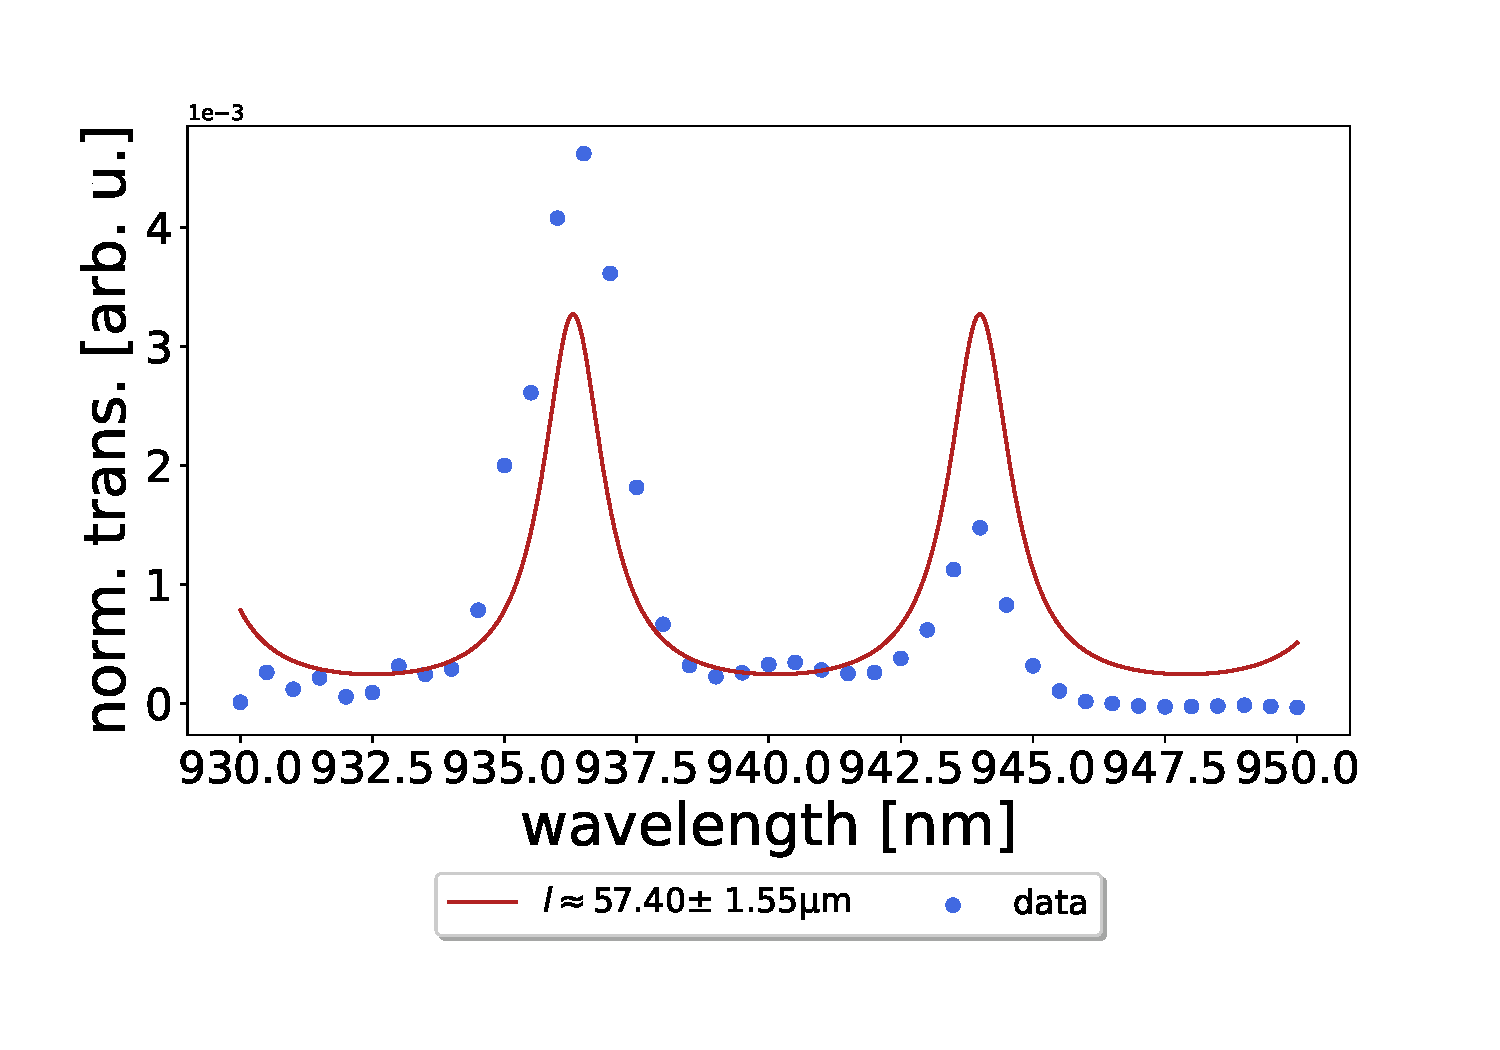
\includegraphics[width=\textwidth]{figures/60um_M5_FSR_fit.pdf}
        \caption{}
        \label{fig:short_single_fano_FSR}
    \end{subfigure}
    \begin{subfigure}[b]{0.49\textwidth}
        \centering
        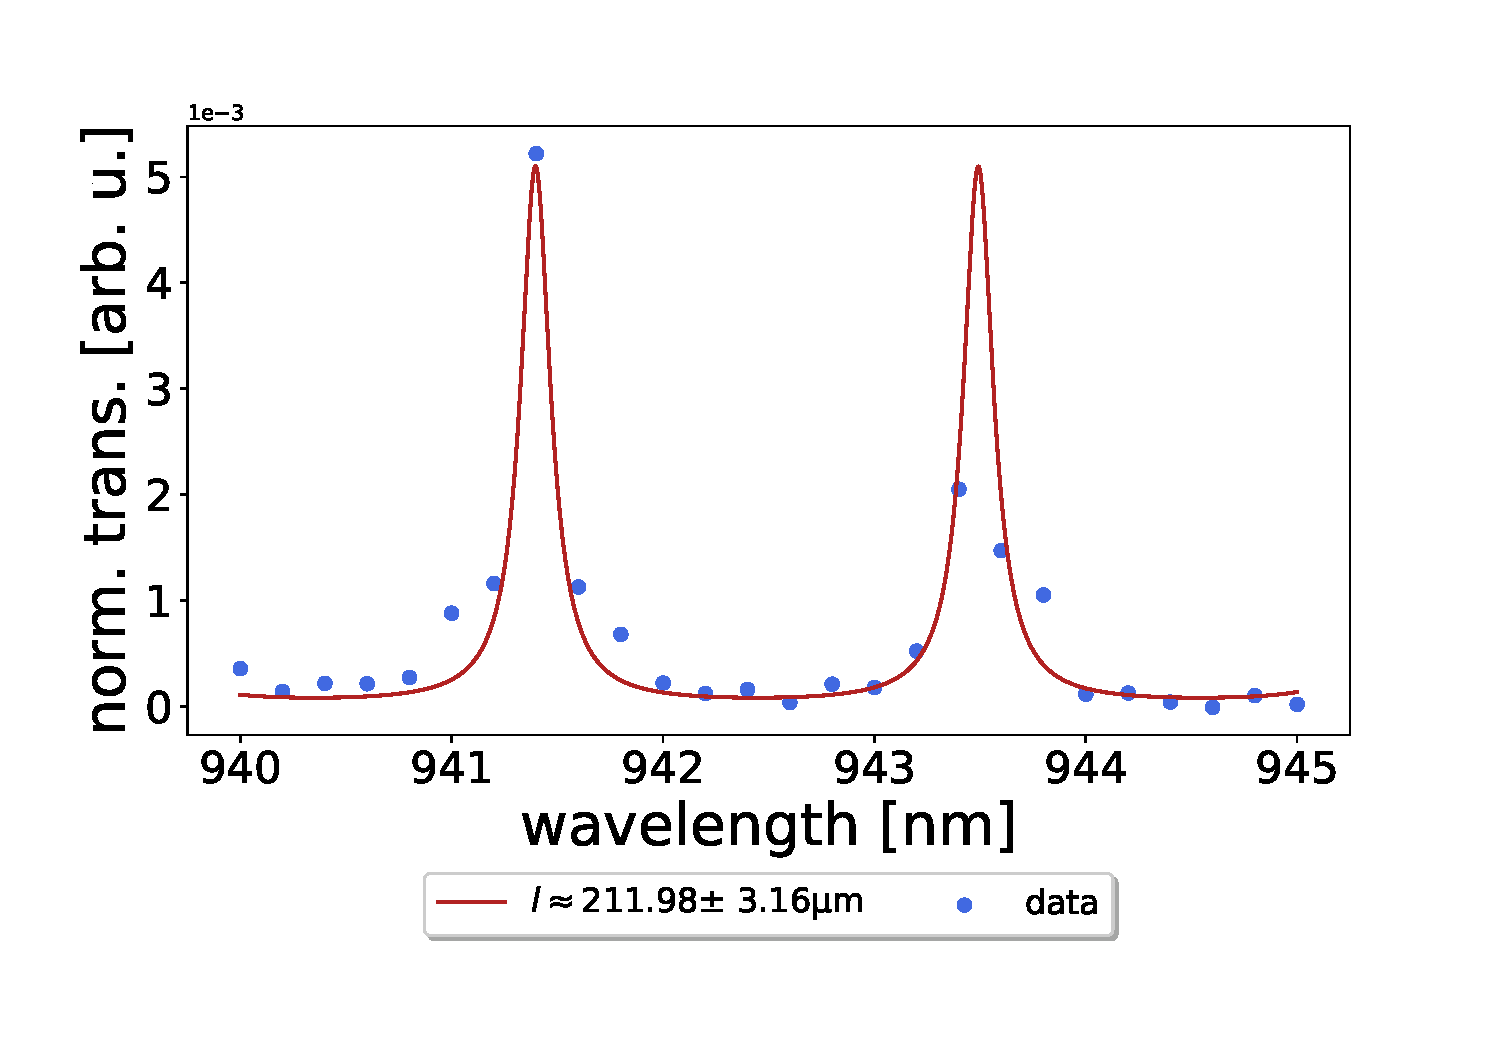
\includegraphics[width=\textwidth]{figures/220um_M5_FSR_fit.pdf}
        \caption{}
        \label{fig:long_single_fano_FSR}
    \end{subfigure}
\end{figure}

\begin{figure}[h!]
    \centering
    \begin{subfigure}[b]{0.49\textwidth}
        \centering
        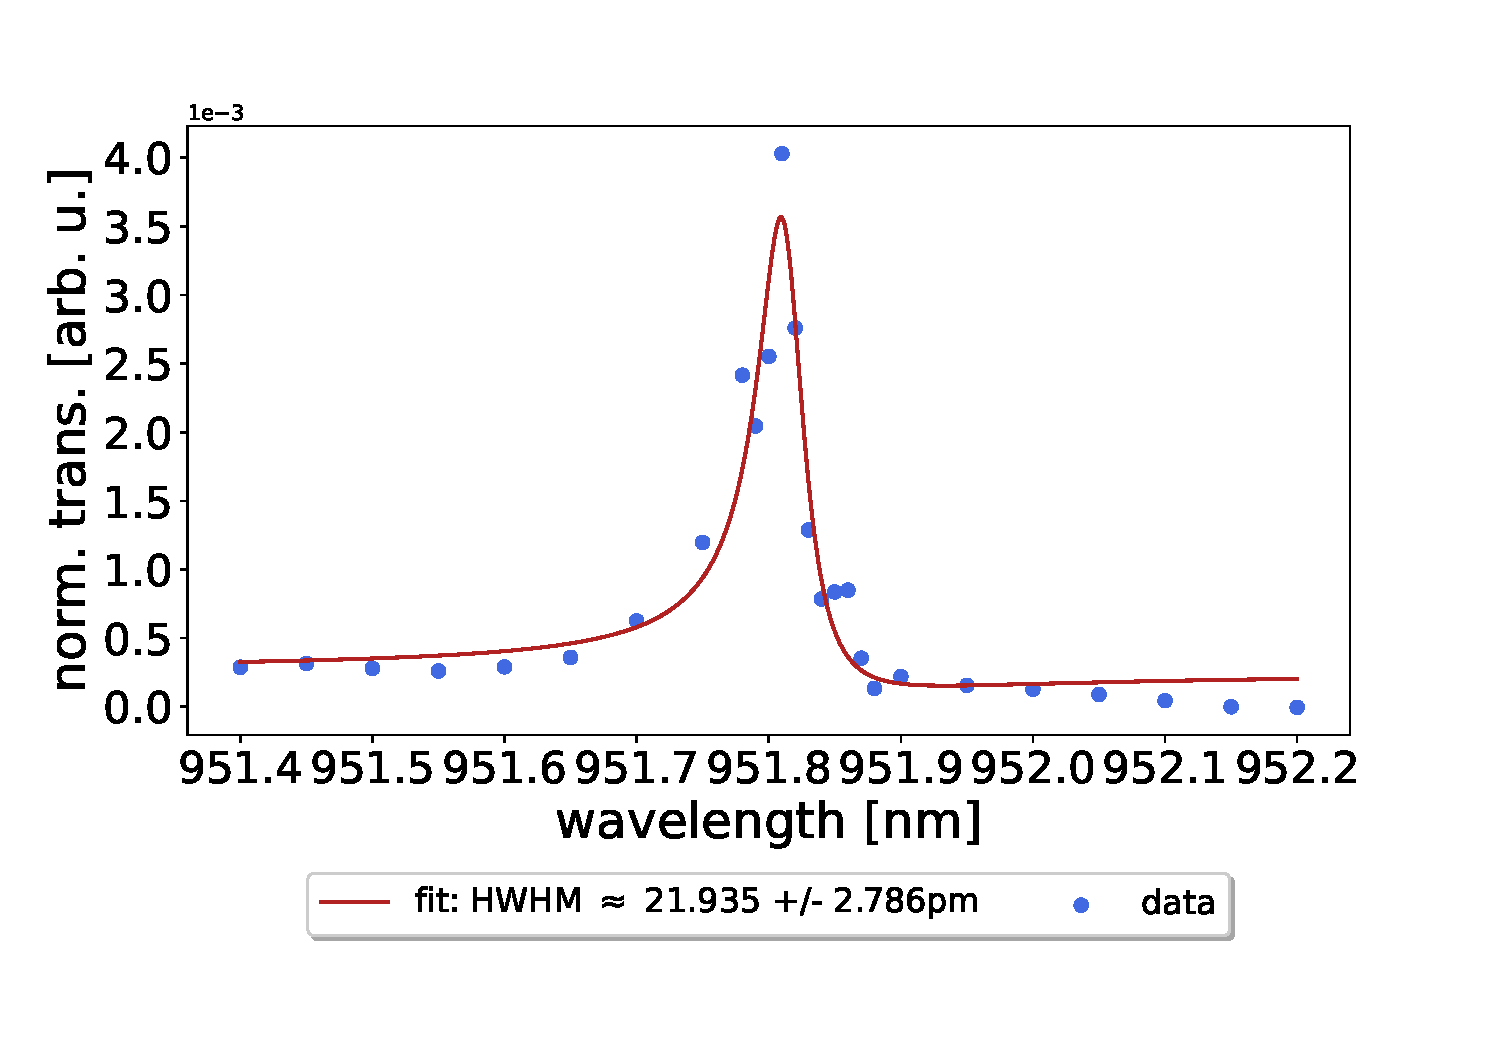
\includegraphics[width=\textwidth]{figures/60um_M5_fit_1.pdf}
        \caption{}
        \label{fig:short_single_fano_trans}
    \end{subfigure}
    \begin{subfigure}[b]{0.49\textwidth}
        \centering
        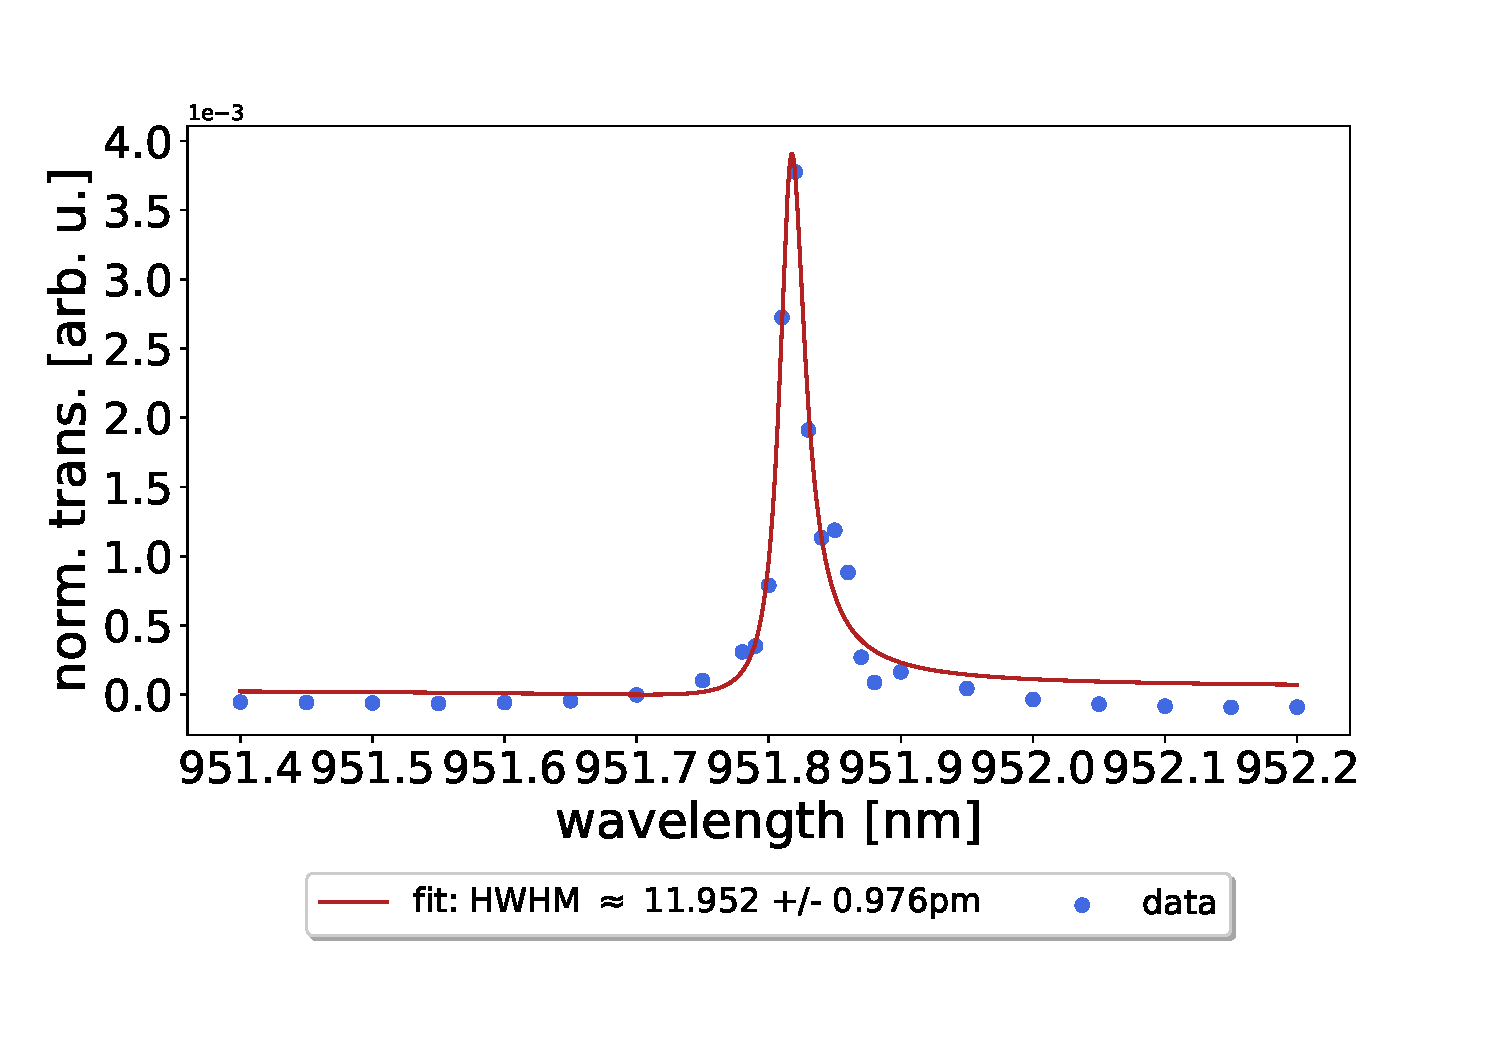
\includegraphics[width=\textwidth]{figures/220um_M5_fit_4.pdf}
        \caption{}
        \label{fig:long_single_fano_trans}
    \end{subfigure}
\end{figure}

\begin{figure}[h!]
    \centering
    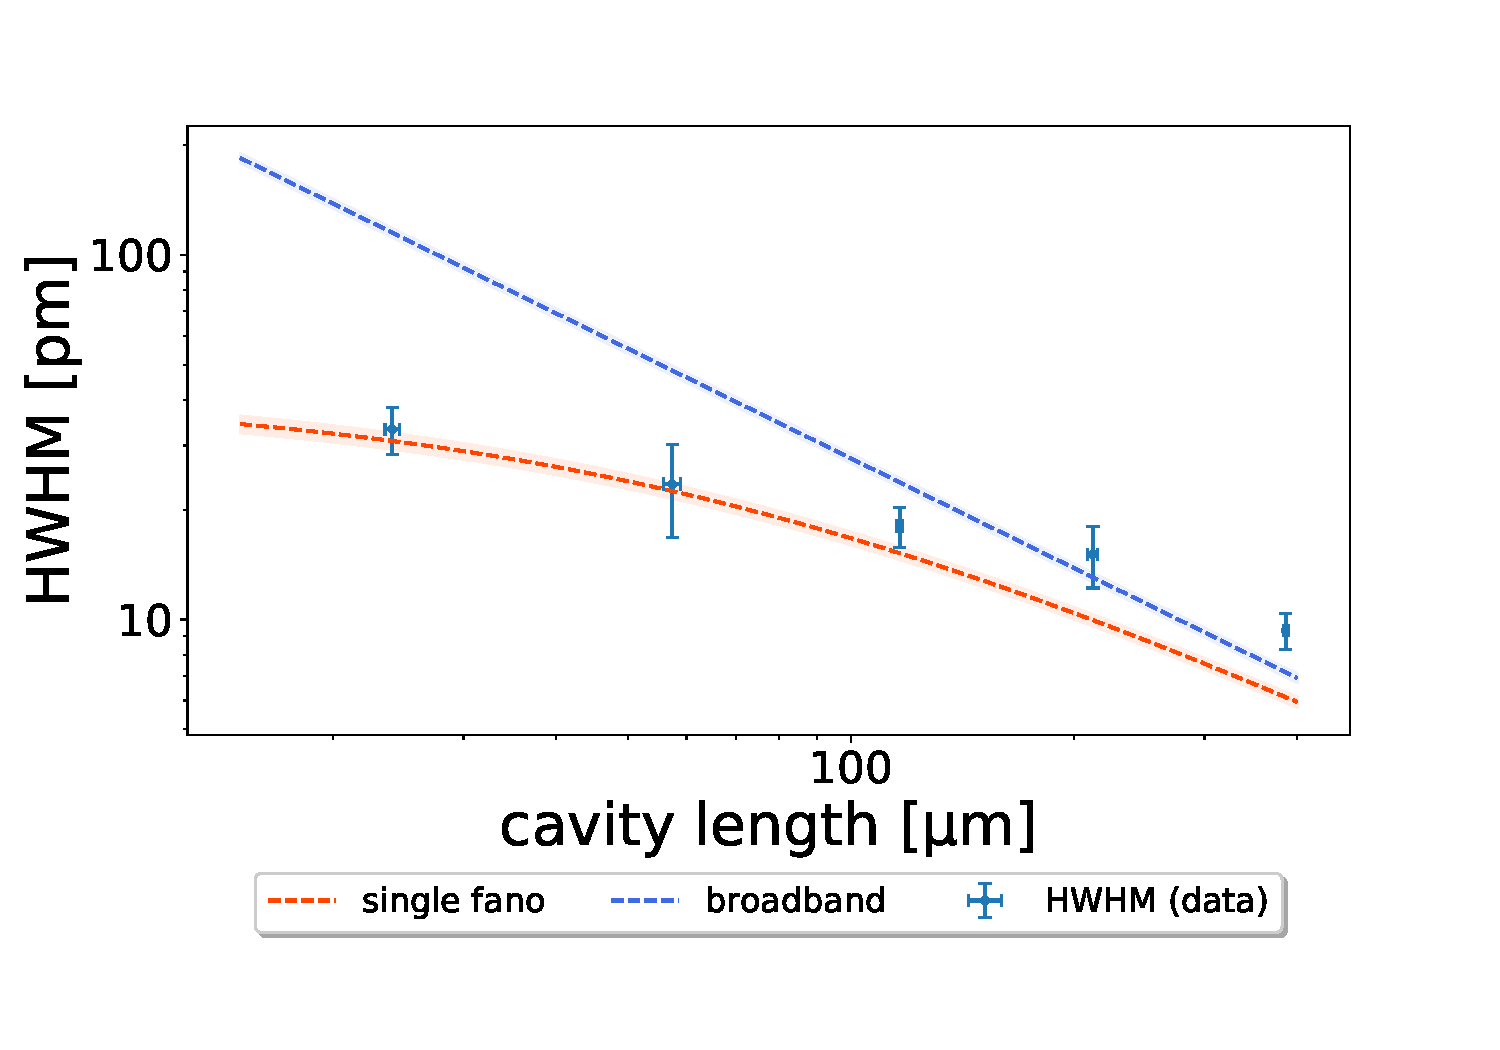
\includegraphics[width=0.7\textwidth]{figures/HWHM_vs_cavity_length_single_fano.pdf}
    \caption{}
    \label{fig:HWHM_vs_time_single_fano_data}
\end{figure}

\subsection{The double Fano cavity}

\subsubsection{Realizing the double fano model}

Figures: 
\begin{itemize}
    \item Fit of the double fano model (long + short cavity)
\end{itemize}

\subsubsection{Double fano off-resonance Fabry-Perot cavity}

Figures:
\begin{itemize}
    \item Off-resonance double fano transmission as a function of wavelength (show that the off resonance transmission goes close to 100 percent for a well-aligned cavity).
\end{itemize}

\subsubsection{The double fano linewidth}

Figures: 
\begin{itemize}
    \item "Semi-short" scan data, fit to the double fano transmission model. 
    \item Short scan data, fit to the Fano function (for measuring linewidth).
    \item Linewidth as a function of cavity length (compare double fano, single fano and broadband cavitites).
\end{itemize}

